\subsection{ソフトウェア設計の基礎}

ソフトウェア設計の基礎は、設計を理解するための概念、用語、判断基準である。初学者にとって重要なのは、設計を「コードを書く前の一工程」と狭く見るのではなく、「問題を解決可能な形へ変換する思考」として見ることである。

\subsubsection{設計思考}

\term{設計思考}{Design Thinking} は、必要や問題を理解し、それに対する解決策を考える思考である。設計対象はソフトウェアに限らない。建築、工業製品、組織、業務手順など、人が目的を持って作るものには設計が関わる。

ソフトウェア設計で重要なのは、問題と解決策を表す語彙を作ることである。ソフトウェアは、物理的な材料を削って作るものではなく、概念、名前、規則、手続き、データ、インタフェースを組み合わせて作る。したがって、設計は言語的な活動でもある。

設計思考は、次の五段階として理解できる。
\begin{enumerate}
  \item 目的や目標を明確にする。
  \item その目的を達成する概念的な構造を考える。
  \item 概念構造を実現する仕組みを考える。
  \item その仕組みを表し、利用するための記法や語彙を作る。
  \item 具体的な問題文脈で記法を使い、目的を達成する。
\end{enumerate}

\begin{definitionbox}
設計思考とは、問題を理解し、制約の中で複数の解決策を考え、根拠を持って選び、表現可能な形へまとめる思考である。
\end{definitionbox}

\begin{figure}[htbp]
\centering
\IfFileExists{assets/generated_figures/ch03/fig-ch03-02.png}{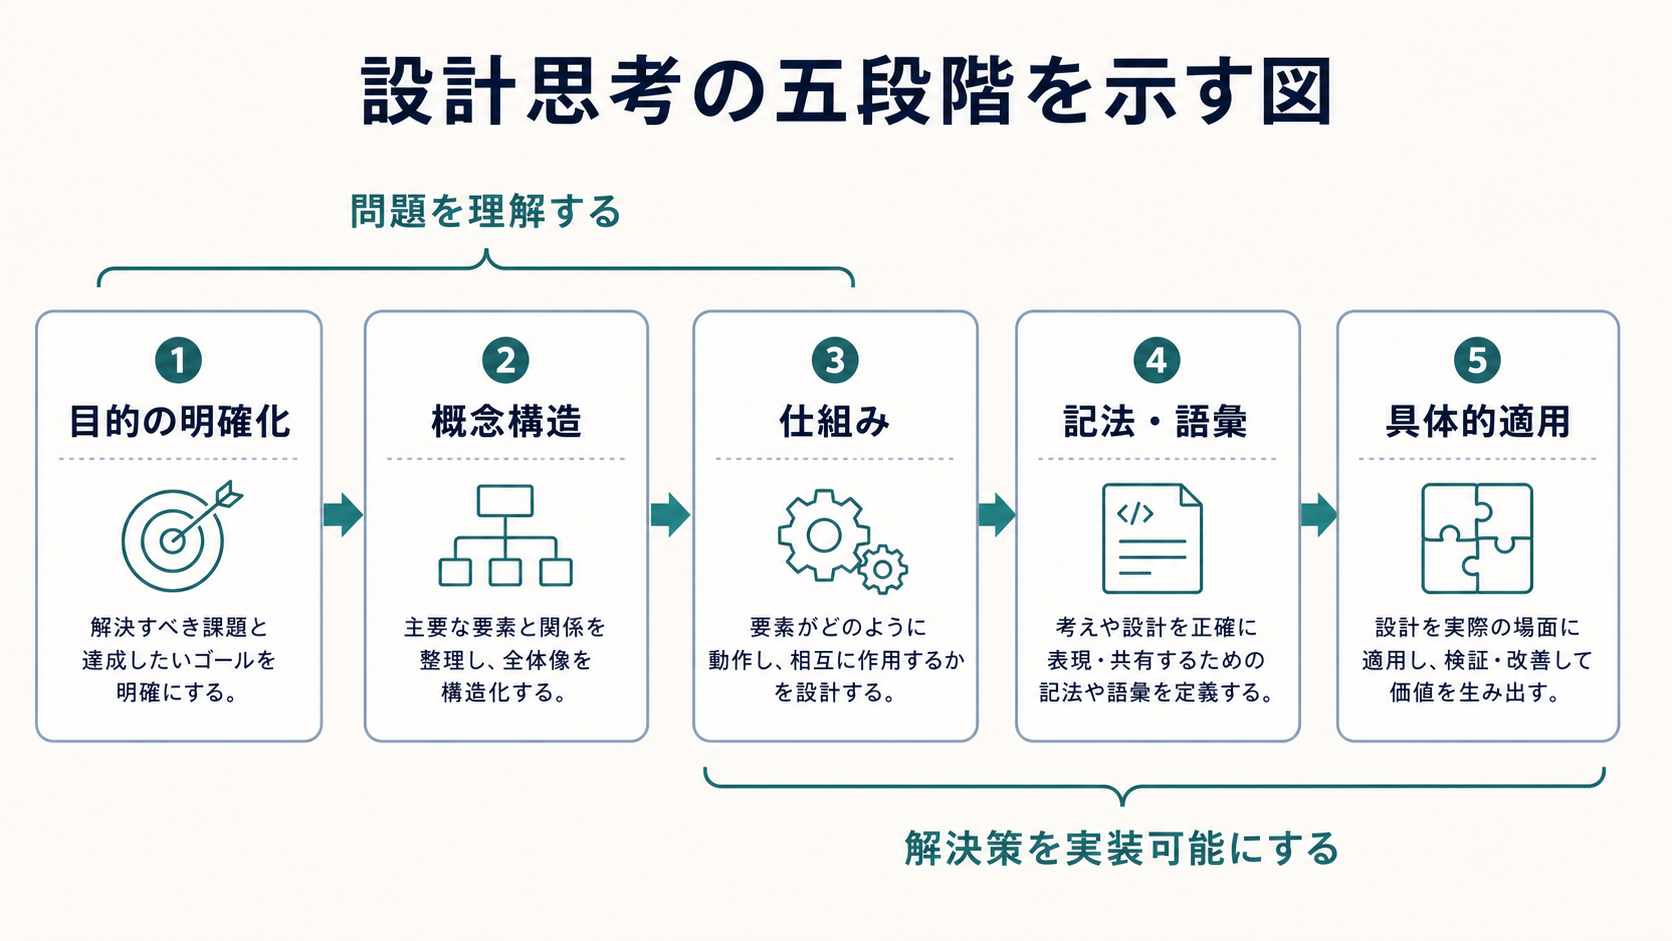
\includegraphics[width=0.96\linewidth]{assets/generated_figures/ch03/fig-ch03-02.png}}{\fbox{\parbox[c][48mm][c]{0.9\linewidth}{\centering 画像生成待ち\\設計思考の五段階を示す図}}}
\caption{設計思考の五段階を示す図}
\label{fig:ch03-02}
\end{figure}

\subsubsection{ソフトウェア設計の文脈}

ソフトウェア設計は、開発ライフサイクルの中で孤立して存在しない。要求、アーキテクチャ、実装、テスト、保守と強くつながっている。

\begin{itemize}
  \item \textbf{要求との関係}：要求は、設計が解くべき問題を示す。設計は、要求を実装可能な構造と振る舞いへ変換する。
  \item \textbf{アーキテクチャとの関係}：アーキテクチャが定められている場合、それは設計の制約となる。主要構成要素、接続、API、採用すべきスタイルやパターン、設計原則などを制約する。
  \item \textbf{実装との関係}：設計は、実装者が何を作るべきかを示す案内である。実装者がコードを読む前に、部品の責務やインタフェースを理解できることが望ましい。
  \item \textbf{テストとの関係}：設計は、テスト戦略とテストケースの土台になる。設計要素が要求をどう満たすかが明らかであれば、テストの観点も作りやすい。
\end{itemize}

設計の形式性は、プロジェクトによって異なる。安全性が重要なシステムでは、設計記述を厳密に残す必要がある。一方、小規模な探索的開発では、簡潔なモデルやコードそのものが設計記録の中心になる場合もある。ただし、どの場合でも、関係者が設計判断を理解できることが重要である。

\begin{figure}[htbp]
\centering
\IfFileExists{assets/generated_figures/ch03/fig-ch03-03.png}{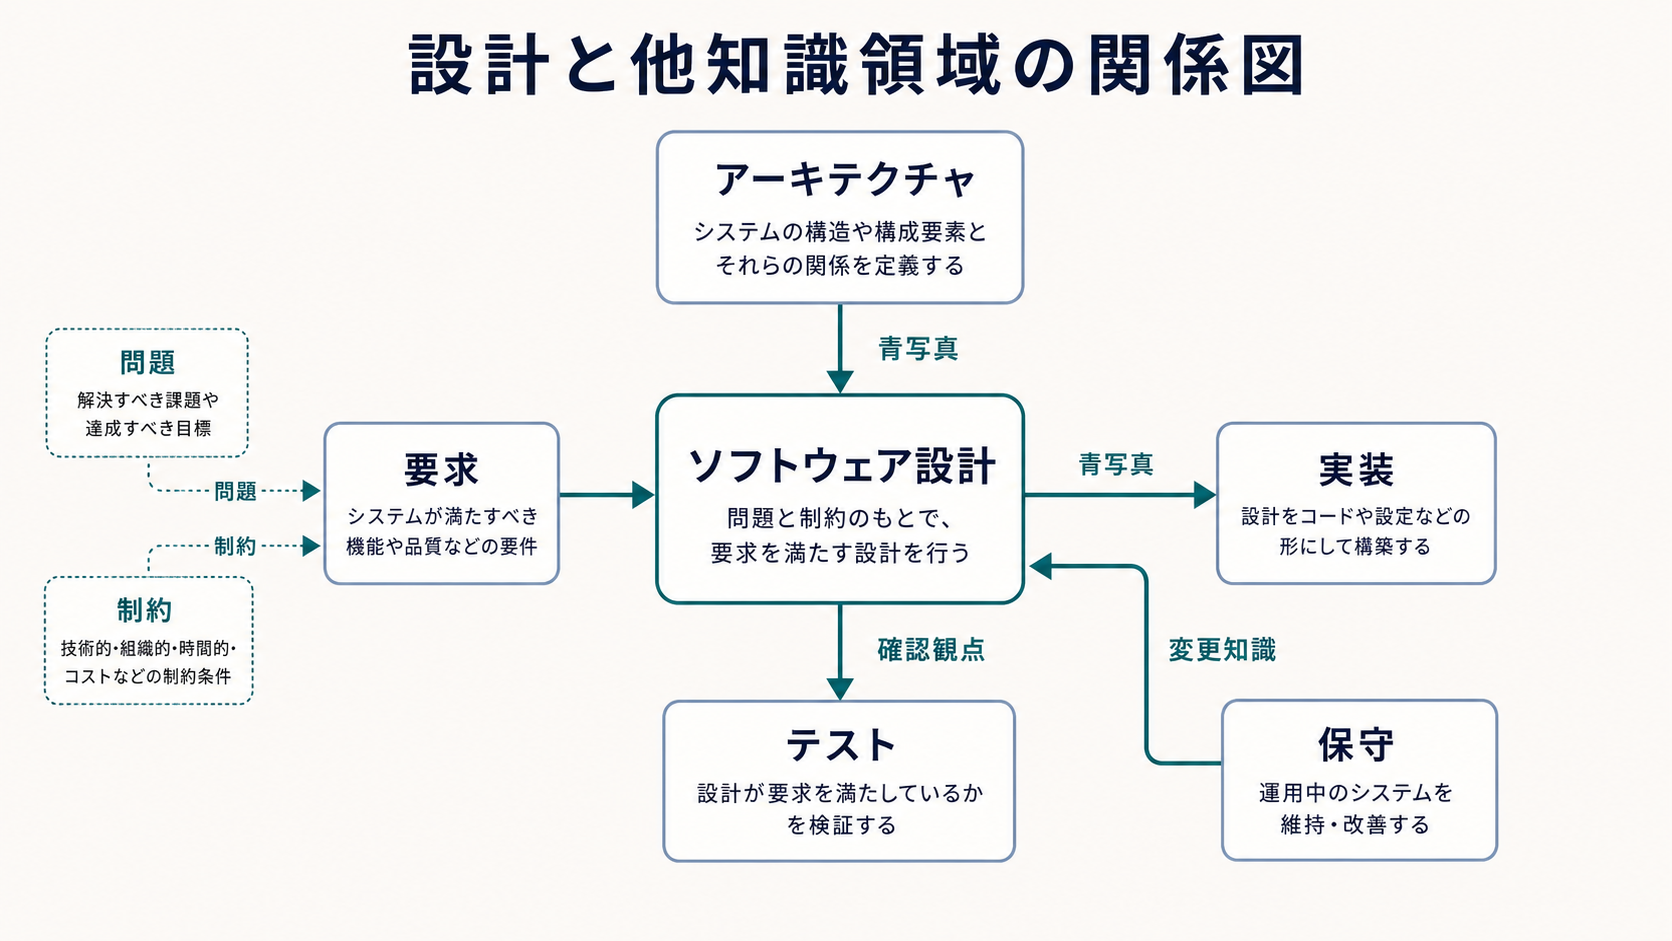
\includegraphics[width=0.96\linewidth]{assets/generated_figures/ch03/fig-ch03-03.png}}{\fbox{\parbox[c][48mm][c]{0.9\linewidth}{\centering 画像生成待ち\\設計と他知識領域の関係図}}}
\caption{設計と他知識領域の関係図}
\label{fig:ch03-03}
\end{figure}

\subsubsection{ソフトウェア設計の主要論点}

設計では、多くの論点を同時に扱う必要がある。代表的な論点は、性能、セキュリティ、信頼性、使いやすさ、保守容易性などの品質である。また、ソフトウェアをどのような構成要素へ分けるか、それらをどう接続するか、どの単位で責務を持たせるかも重要である。

設計論点には、機能そのものではないが、システム全体に影響するものもある。たとえば、ログ、認証、監査、例外処理、キャッシュ、トランザクション、セキュリティ確認などは、多くの機能に横断的に関わる。こうした論点は\term{横断的関心事}{crosscutting concern} と呼ばれる。

\begin{pointbox}{注意}
横断的関心事を場当たり的に実装すると、同じ処理が各所に重複し、変更時に漏れが起きやすくなる。設計段階で共通方針を決めることが重要である。
\end{pointbox}

\subsubsection{ソフトウェア設計原則}

設計原則は、設計中の判断に方向を与える基本的な考え方である。原則は、特定のプログラミング言語や開発手法だけに依存しない。むしろ、複雑な問題を扱うための共通の知恵である。

\par\smallskip\noindent\refstepcounter{table}\label{tab:ch03-03}\textbf{表 \thetable: 第03章 ソフトウェア設計 表03}\par\smallskip
\begin{longtable}{L{34mm}L{55mm}L{76mm}}
\toprule
\textbf{原則} & \textbf{意味} & \textbf{実務で見ること} \\
\midrule
\endhead
抽象化 & 目的に関係する情報だけを示し、不要な詳細を隠す。 & 利用者、設計者、実装者が必要な詳細水準だけを見られるか。 \\
関心事の分離 & 異なる関心を分けて扱う。 & 業務処理、認証、ログ、表示、保存などが混ざりすぎていないか。 \\
モジュール化 & 大きなソフトウェアを小さな部品へ分ける。 & 各部品の責務が明確で、独立して理解・変更できるか。 \\
カプセル化・情報隠蔽 & 内部詳細を隠し、必要なインタフェースだけを見せる。 & 外部が内部データ構造や実装順序に依存していないか。 \\
インタフェースと実装の分離 & 外部に見せる契約と内部実装を分ける。 & 実装を変えても、利用側の変更が少なく済むか。 \\
結合度 & 部品同士の依存の強さである。 & ひとつの部品変更が多数の部品変更を引き起こさないか。 \\
凝集度 & ひとつの部品内の要素がどれだけ関連しているかである。 & ひとつの部品が複数の無関係な責務を抱えていないか。 \\
一貫性 & 名前、記法、順序、インタフェースなどをそろえる。 & 似た問題に似た解決策を使っているか。 \\
完全性 & 重要な特徴や要求を漏らさない。 & 通常時、例外時、境界条件、状態、モードが考慮されているか。 \\
検証可能性 & 要求や制約を満たすか確認できる。 & 設計からテスト、レビュー、分析が可能か。 \\
倫理的配慮 & 人権、福祉、透明性、説明責任、悪用可能性などを考慮する。 & AI、自律システム、社会的影響があるシステムで設計上の配慮があるか。 \\
\bottomrule
\end{longtable}

特に、結合度と凝集度は初学者が最初に押さえるべき設計観点である。一般に、よい設計は、部品間の結合度を低くし、部品内の凝集度を高くする。結合度が高いと変更の影響が広がる。凝集度が低いと、部品が何を担当しているのか理解しにくくなる。

\begin{pointbox}{重要}
設計原則は、単独で使うものではない。抽象化、関心事の分離、モジュール化、カプセル化、低結合、高凝集は互いに支え合う。
\end{pointbox}

\begin{figure}[htbp]
\centering
\IfFileExists{assets/generated_figures/ch03/fig-ch03-04.png}{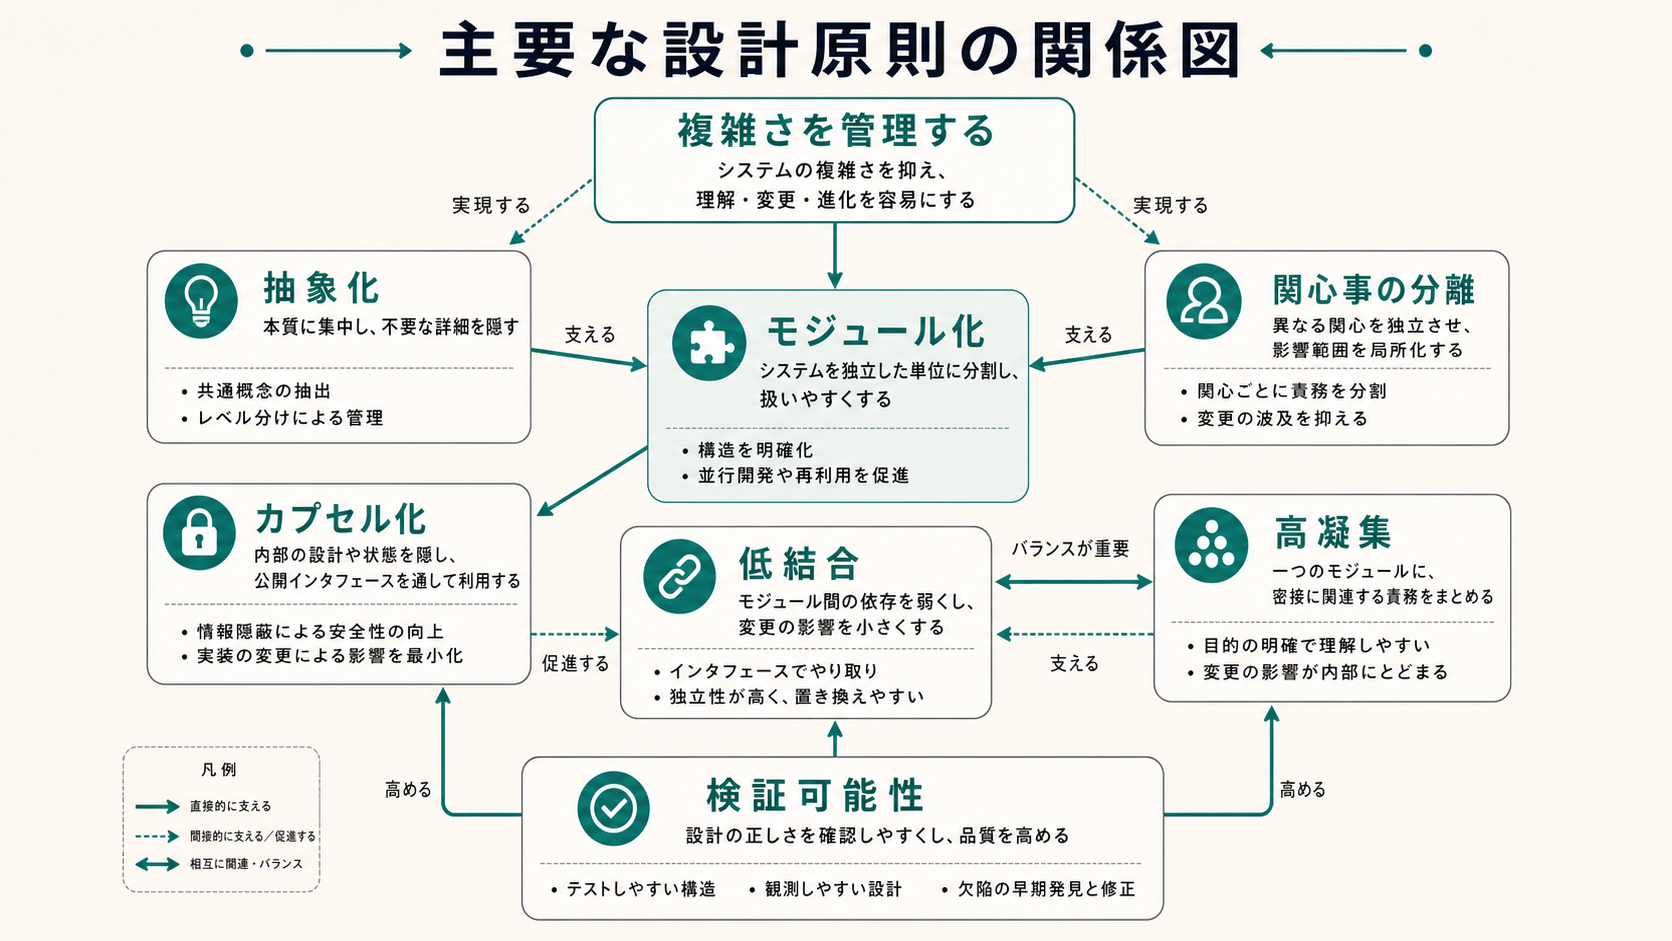
\includegraphics[width=0.96\linewidth]{assets/generated_figures/ch03/fig-ch03-04.png}}{\fbox{\parbox[c][48mm][c]{0.9\linewidth}{\centering 画像生成待ち\\主要な設計原則の関係図}}}
\caption{主要な設計原則の関係図}
\label{fig:ch03-04}
\end{figure}
